\lhead{\begin{tikzpicture}[remember picture, overlay]
    \node [anchor=100,inner sep=0] (imagenIZQUIERDA) at (current page header area.north){
\includegraphics[width=18cm]{img/Encabezado.PNG}};
    \end{tikzpicture}}
    \rhead{Autor: primerApellido-segundoApellido}
    \rfoot{\begin{tikzpicture}[remember picture, overlay]
    \node [anchor=140,inner sep=0] (imagenDERECHA) at (current page footer area.south){
\includegraphics[width=18cm]{img/Foot.PNG}};
    \end{tikzpicture}}
    %----------------------------------------------------------------------------------------
    \lfoot{ \thepage}
    % \renewcommand{\labelenumi}{\alph{enumi}.)} 
    %----------------------------------------------------------------------------------------
    %----------------------------------------------------------------------------------------
    %	TITLE SECTION
    %----------------------------------------------------------------------------------------
    
    \setlength{\droptitle}{-5\baselineskip} % Move the title up
    \title{\textbf{Estudio de tiempos y movimientos en el ensamble de un circuito electrónico utilizando diferentes métodos para su optimización}} % Article title
    
     \author{ 
     \textsc{Sanchez Nava Edwin Ernesto}\\ 
    %  Afiliación:
     \texttt{ ITQ Campus Qro } \\ 
     \texttt{Instituto Tecnológico de Queretaro } \\ 
     \texttt{Queretaro, Mexico}\\ 
     \texttt{l22140867@queretaro.tecnm.mx} 
     \and 
     \textsc{Apellidos, Nombre/s}\\ 
    %  Afiliación:
     \texttt{ Nombre Instituto } \\ 
     \texttt{Nombre de la Organización } \\ 
     \texttt{Ciudad y País}\\ 
     \texttt{Correo electrónico} 
    }
    
    
    %----------------------------------------------------------------------------------------
    
    % \begin{document}
    
    % Print the title
    \maketitle
    \thispagestyle{fancy}
    
    %----------------------------------------------------------------------------------------
    %	ARTICLE CONTENTS
    %----------------------------------------------------------------------------------------
    
    % \section*{Resumen}
    % \textit{Palabras clave:}
    % El resumen (ancho de página) deberá contener entre 100 y 200 palabras tipo Adobe Devangari 11 puntos.
    
    \begin{abstract}
    \noindent 
    El resumen (ancho de página) deberá contener entre 100 y 200 palabras tipo Adobe Devangari 11 puntos.
    
    \end{abstract}
    % 
    % 
    \textbf{\textit{Palabras clave}}: {First keyword should be the corresponding to the research area according with the authors guide. Maximum of 6 keywords.}
    % \keywords{First keyword should be the corresponding to the research area according with the authors guide. Maximum of 6 keywords.}
    
    \section{Introducción}
    
    % Define estudio de tiempos y movimientos: 
        % define que es ensamble:
        % define que es circuito electronico:
        % define el metodo de tiempos predeterminados: 
        % define optimización: Buscar la mejor manera de realizar una actividad.
        El estudio de tiempos y movimientos es una disciplina fundamental en la ingeniería industrial, que se enfoca en analizar y mejorar la eficiencia de los procesos productivos. En el contexto del ensamble de circuitos electrónicos, este estudio cobra una relevancia particular debido a la naturaleza precisa y delicada de las operaciones involucradas.
    
        El ensamble de circuitos electrónicos implica la manipulación de componentes pequeños y delicados, así como la realización de conexiones precisas. Cada paso en este proceso requiere una cuidadosa consideración para garantizar la calidad del producto final y optimizar la eficiencia de producción.
    
        En este sentido, el presente estudio se propone explorar diferentes métodos y técnicas para analizar, medir y mejorar los tiempos y movimientos en el ensamble de circuitos electrónicos. Desde enfoques clásicos como el análisis de tiempos predeterminados y la cronometría de movimientos, hasta herramientas más avanzadas como la simulación por computadora y la optimización algorítmica, se buscará identificar oportunidades de mejora en la productividad y la calidad.
        
        \section{Justificación}
    
        El estudio de tiempos y movimientos en el ensamble de circuitos electrónicos es crucial debido a varios factores clave que afectan tanto la eficiencia operativa como la calidad del producto final. A continuación se presentan algunas razones que respaldan la necesidad de llevar a cabo este estudio utilizando diferentes métodos para su optimización:
        \begin{itemize}
            \item Optimización de recursos: El ensamble de circuitos electrónicos implica el uso de recursos costosos y delicados, como componentes electrónicos y equipos especializados. Optimizar los tiempos y movimientos ayuda a maximizar la utilización de estos recursos, minimizando el desperdicio y reduciendo los costos de producción.
            \item  Al identificar y eliminar actividades innecesarias o redundantes, así como optimizar los procesos de ensamble, se puede aumentar la productividad de la línea de producción. Esto se traduce en una mayor cantidad de circuitos electrónicos ensamblados en un período de tiempo dado, lo que mejora la capacidad de respuesta ante la demanda del mercado.
            \item Calidad del producto: Los tiempos y movimientos ineficientes pueden contribuir a errores de ensamble, mal funcionamiento de los circuitos electrónicos y defectos en el producto final. Al optimizar estos aspectos, se reduce la probabilidad de errores y se mejora la calidad del producto, lo que conduce a una mayor satisfacción del cliente y una reputación positiva de la marca.
            \item Ergonomía y seguridad laboral: Un estudio detallado de los movimientos realizados por los operarios en el ensamble de circuitos electrónicos permite identificar y corregir posturas incómodas o movimientos repetitivos que pueden causar fatiga o lesiones laborales. Mejorar la ergonomía en el lugar de trabajo no solo aumenta el bienestar de los empleados, sino que también puede aumentar la eficiencia y la precisión en las tareas realizadas.
            \item  En un mercado globalizado y altamente competitivo, las empresas que pueden producir circuitos electrónicos de manera más eficiente y con una calidad superior tienen una ventaja significativa. El estudio de tiempos y movimientos, junto con su optimización, ayuda a las empresas a mejorar su competitividad al reducir costos, mejorar la calidad y aumentar la capacidad de respuesta a las demandas del mercado.
        \end{itemize}
    
        %La optimización de procesos de ensamble es fundamental para mejorar la eficiencia y la productividad en entornos industriales. Mediante un estudio de tiempos detallado, podemos identificar áreas de oportunidad para reducir los tiempos de producción, minimizar los tiempos muertos y mejorar la calidad del producto final. Este proyecto tiene como objetivo principal aplicar técnicas de ingeniería industrial para analizar y mejorar el proceso de ensamble, lo que resultará en una reducción de costos, un aumento en la producción y una mayor satisfacción del cliente. Al entender mejor cómo se lleva a cabo el ensamble y dónde se pueden realizar mejoras, podemos optimizar el flujo de trabajo, eliminar cuellos de botella y aumentar la eficiencia operativa. En última instancia, este proyecto contribuirá significativamente a la competitividad y rentabilidad de nuestra empresa en un mercado cada vez más exigente y competitivo.
    
        \begin{itemize}
           \item Se debe de describir lo que se requiere, lo que se necesita o lo que se demanda en la actualidad con un enfoque global pero terminar con menciones a temas locales o nacionales.
           % \item Debe de tener Referencias científicas, URL, tesis, etc.
        \end{itemize}
        % 
        % 
        \section{Descripción del problema}
        El problema del estudio de tiempos y movimientos en el ensamble de circuitos electrónicos abarca una serie de desafíos complejos que pueden afectar tanto la eficiencia operativa como la calidad del producto final.
        En resumen, el problema del estudio de tiempos y movimientos en el ensamble de circuitos electrónicos abarca una serie de desafíos que afectan la eficiencia, la calidad, la seguridad laboral y la rentabilidad del proceso. La aplicación de diferentes métodos de optimización es fundamental para abordar estos desafíos de manera efectiva y promover la excelencia en la producción de circuitos electrónicos.
    
        % 
        % 
        \section{Fundamentación teórica}
    
        La fundamentación teórica del estudio de tiempos y movimientos en el ensamble de un circuito electrónico se basa en varios principios y conceptos fundamentales de la ingeniería industrial y la gestión de operaciones. Aquí hay una descripción de algunos de los aspectos teóricos clave:
        \begin{itemize}
            \item Análisis de tiempos: Este método implica medir y registrar el tiempo requerido para completar cada tarea individual en el proceso de ensamble. Se basa en la idea de que entender cómo se distribuye el tiempo entre las diferentes actividades permite identificar oportunidades de mejora y eliminar actividades innecesarias o redundantes. El análisis de tiempos proporciona una base cuantitativa para evaluar la eficiencia del proceso y diseñar intervenciones de mejora.
            \item Cronometraje de movimientos: Este enfoque se centra en analizar y mejorar los movimientos físicos realizados por los trabajadores durante el ensamble de circuitos electrónicos. Se basa en los principios de ergonomía y biomecánica para identificar movimientos ineficientes, repetitivos o que puedan causar fatiga o lesiones. Al optimizar los movimientos, se puede mejorar la eficiencia del proceso y reducir el riesgo de lesiones laborales.
            \item Estudio de métodos: Este método implica analizar y comparar diferentes métodos o técnicas utilizadas para realizar una tarea específica en el ensamble de circuitos electrónicos. Se busca identificar el método más eficiente que permita completar la tarea de manera rápida, precisa y segura. El estudio de métodos puede involucrar la evaluación de herramientas, equipos, diseños de estaciones de trabajo y procedimientos de trabajo.
        \end{itemize}
        % 
        % 
        \section{Hipótesis}
    
        Aquí hay algunas hipótesis que podrían plantearse en el contexto del estudio de tiempos y movimientos en el ensamble de un circuito electrónico:
        \begin{itemize}
            \item  Se hipotetiza que la aplicación de técnicas de análisis de tiempos y movimientos, junto con métodos de optimización, permitirá reducir significativamente los tiempos de ciclo en el ensamble de circuitos electrónicos, mejorando así la eficiencia del proceso.
            \item Se plantea que al optimizar los movimientos y métodos de ensamble, se reducirán los errores y defectos en el producto final, lo que resultará en una mejora general en la calidad de los circuitos electrónicos ensamblados.
            \item Se plantea que al analizar y optimizar los movimientos realizados por los trabajadores durante el ensamble de circuitos electrónicos, se mejorará la ergonomía de las estaciones de trabajo, reduciendo la fatiga y el riesgo de lesiones laborales.
        \end{itemize}
        Estas hipótesis proporcionan un marco inicial para el estudio y la investigación sobre la optimización del ensamble de circuitos electrónicos a través del análisis de tiempos y movimientos, y pueden servir como base para la formulación de objetivos y la evaluación de resultados.
        % 
        % 
        \section{Objetivo}
            El objetivo principal del estudio de tiempos y movimientos en el ensamble de un circuito electrónico es mejorar la eficiencia, la calidad y la seguridad del proceso de producción. Para lograr este objetivo, se pueden establecer los siguientes objetivos específicos:
    
        \subsection{Objetivos específicos }
    
        \begin{itemize}
            \item Reducir los tiempos de ciclo: Mediante la identificación y eliminación de actividades innecesarias, así como la optimización de los movimientos y métodos de ensamble, se busca reducir el tiempo total requerido para ensamblar un circuito electrónico, aumentando así la productividad y la capacidad de respuesta del proceso.
            \item Mejorar la calidad del producto: Al optimizar los tiempos y movimientos, se busca reducir la probabilidad de errores y defectos en el producto final. Esto se logra mediante la estandarización de procedimientos, la mejora de la precisión en el ensamble y la implementación de controles de calidad efectivos.
            \item Optimizar el uso de recursos: Se pretende utilizar de manera más eficiente los recursos disponibles, como el tiempo de trabajo, el espacio de trabajo, los equipos y los materiales. Esto implica minimizar el desperdicio y maximizar la utilización de los recursos para reducir los costos de producción y aumentar la rentabilidad.
            \item Promover la mejora continua: El estudio de tiempos y movimientos proporciona una base sólida para la identificación de oportunidades de mejora y la implementación de cambios efectivos en el proceso de ensamble de circuitos electrónicos. Se busca fomentar una cultura de mejora continua, donde se busque constantemente optimizar el proceso y adaptarse a los cambios en el entorno operativo. 
    
        \end{itemize}
    
        %Son actividades orientadas al cumplimiento del objetivo general. Se establecen con verbos activos en infinitivo. Son parte de la acción encaminada a probar la hipótesis. Éstos deben ser precisos, y en lo posible evitar aspectos metodológicos.
        % 
        % 
        \section{Cuerpo (Metodología, modelo matemático, etc.)}
    
        %Cada estrategia metodológica se establece acorde a cada objetivo, y por tanto deberá ser desglosada precisada y ordenada claramente. En consecuencia cada objetivo que se presentó en forma de verbo en infinitivo deberá determinar una estrategia en forma de adverbio. Ej. Desarrollar…Desarrollo. Son las actividades ordenadas que tienen como finalidad la prueba de la hipótesis. 
    
    
    
         Componentes necesarios: 
        \begin{itemize}
    
        \item ESP32 (controlador)
        \item Potenciómetro (para ajustar el valor a mostrar)
        \item Pantalla LCD 16x2 (para mostrar el valor)
        \item Cable USB tipo c (para alimentar el ESP32 desde un multicontacto)
        \item Protoboard o placa de circuito impreso
        \item Cables de conexión (jumpers)
        \item Resistencias (si es necesario para la pantalla LCD)
        \item Capacitores (si es necesario para el ESP32)
    
        \end{itemize}
    
        Procedimiento de ensamblaje:
        \begin{itemize}
    
        \item Conecta el ESP32 a la protoboard o placa de circuito impreso. Asegúrate de conectar los pines de alimentación (VCC y GND) y los pines de comunicación.
        \item Conecta el potenciómetro a la protoboard. Conecta los extremos del potenciómetro a VCC y GND, y el terminal central a un pin analógico del ESP32.
        \item Conecta la pantalla LCD a la protoboard. Si es necesario, conecta las resistencias y capacitores según las especificaciones del fabricante. Luego, conecta los pines de datos (por ejemplo, los pines de datos seriales o los pines de bus I2C) y los pines de control (como el pin de habilitación y el pin de selección de línea) al ESP32.
        \item Conecta el cable USB desde el multicontacto a una fuente de alimentación adecuada para proporcionar energía al ESP32.
        \item Carga el código necesario en el ESP32 para leer el valor del potenciómetro y mostrarlo en la pantalla LCD. Puedes usar el IDE de Arduino u otro entorno de desarrollo compatible con el ESP32 para escribir y cargar el código.
        \item Verifica la conexión y el funcionamiento del circuito. Asegúrate de que el ESP32 pueda leer correctamente el valor del potenciómetro y mostrarlo en la pantalla LCD.
    
         %\item Se debe establecer que se habrá de hacer, como, conque, y donde para obtener la información que permita probar la hipótesis.  
        %  \item Se debe desglosar de acuerdo a los objetivos específicos. 
        % \item Se debe establecer una estrategia metodológica por cada objetivo específico. De manera simplista se podría decir que se cambia el verbo en infinitivo por su respectivo adverbio.
        %\item En cada objetivo se debe describir que método, que materiales y que equipo se usará para conseguirlo.
        %\item Se deben tener referencias.
        \end{itemize}
        % 
        % 
        \subsection{Prepara tu documento}
    
        Antes de que comiences a utilizar esta plantilla, es recomendable que prepare la información que contendrá en un archivo aparte. 
        Ten preparadas tus gráficas, así como también las tablas aparte, para que sea más fácil integrarlo. 
        Se recomienda fuertemente el uso de \textbf{formato Enhanced Metafile (.emf) para imágenes y gráficas} de resolución óptima. 
        Finalmente, completa y organiza el contenido antes de darle el formato de esta plantilla. 
    
        \subsection{Acrónimos y Abreviaciones}
    
        Los acrónimos y abreviaciones deberán ser definidos únicamente la primera vez que aparecen en el texto, esto para que el lector entienda lo que significan.
    
        \subsection{Ecuaciones}
    
        Las ecuaciones son una excepción a las especificaciones prescritas de esta plantilla. 
        Deberá determinar si su ecuación debe escribirse o no utilizando la fuente Adobe Devangari. 
        Para crear ecuaciones multinivel, puede ser necesario tratar la ecuación como un gráfico e insertarla en el texto después de aplicar el estilo de la platilla.
        Las ecuaciones serán enumeradas de manera consecutiva, y el número de ecuación, entre paréntesis, se colocan al ras de la derecha, utilizando una tabulación derecha. 
    
        \begin{equation}
            \label{eq1}
            x + y = z 
        \end{equation}
    
        Es importante asegurarse de que los símbolos de la ecuación sean definidos antes o inmediatamente después de la ecuación. Utilice “(1)”, en vez de “Eq. 1” al enumerar las ecuaciones, excepto al principio de una oración: “La ecuación (\ref{eq1}) es…”
    
        \section{Resultados y discusión}
    
        Antes de comenzar a preparar tu artículo, es importante que lea primero la guía del autor, la cual incluye los temas o apartados que son necesarios para tener tu trabajo completo.
        Una vez completada la edición del texto, el documento está listo para el uso de esta plantilla. En este archivo recién creado, resalte todo el contenido e importe el archivo de texto preparado. Ahora esta listo para estilizar su documento.
        En esta sección se deben presentar todo lo obtenido de la sección 2, incluidas deducciones o efectos del desarrollo. También se podrán incluir subsecciones numeradas de la siguiente forma:
    
        \subsection{Autores y Afiliaciones}
    
        Para distinguir las afiliaciones de los autores, utilice superíndices iniciando con el número 1, 2, etc., sucesivamente, esto dependerá de la cantidad de los departamentos a los que estén afiliados los autores. En caso de que todos los autores pertenezcan a una mismo departamento e institución, utilizar sólo el superíndice 1. 
    
        \subsection{Identificar los encabezados}
    
        Se les recuerda a los autores que los encabezados deben de estar conforme los solicita la guía del autor. De ahí se puede adaptar el trabajo para que sea más fácil de entender para el lector.
        Los encabezados organizan los temas sobre una base relacional y jerárquica. Por ejemplo, el título del documento es encabezado del texto principal porque todo el material posterior se relaciona y elabora sobre este tema. 
    
        \subsection{Tablas y Figuras}
    
       
    
        \section{Conclusiones}
    
        Se describe aquí el alcance del trabajo, logros obtenidos y perspectivas para el futuro de este. Se sugiere colocar información cuantitativa obtenida.
    
        \section{Agradecimientos}
    
        Es importante darles su debido reconocimiento a los laboratorios, instituciones, organizaciones, entre otros que han sido participes para la culminación de este trabajo. También es importante mencionar, fondos, proyectos, becas, entre otros que se le han otorgado al o los autores para realizar el trabajo de investigación. Ejemplo: “Los autores agradecen al Concejo Nacional de Ciencia y Tecnología por los recursos otorgados…”
    
        \section*{Referencias}
    
        Para esta platilla, se solicita al autor enumerar las citas de manera consecutiva entre corchetes. 
        La puntuación de la oración que sigues sería %\cite{Mesaelides2011}. 
        Refiérase simplemente al número de referencia, como en %\cite{Morales2012}, no utilice “Ref. [3]” o “referencia [3]” excepto al principio de una oración: “La referencia [3] fue la primera…”
        Enumere las notas al pie por separado en superíndices. Coloque la nota de pie de en la parte inferior de la columna en la que se citó. No coloque notas al pie en la lista de referencias. Utilice letras para las notas al pie de la tabla.
        A menos de que haya tres autores o más; no utilice “et al.”. Los trabajos que no hayan sido publicados, incluso si han sido presentados para su publicación, deben ser citados como “inéditos”. Los trabajos que han sido aceptados para su publicación deben de citarse como “en prensa”. Poner en mayúscula sólo la primera palabra de un título, excepto los nombres propios y los símbolos de elemento. 
    
        Otros ejemplos %\cite{LAAngeles2021}, \cite{LAAngelesConni}. 
    
    \subsection{Tabla de Materiales}
    \begin{table}[H]
        \centering
        \begin{tabular}{|c|c|c|}
        \hline
        Nombre & Imagen & Plano \\
        \hline
        Cable MH & 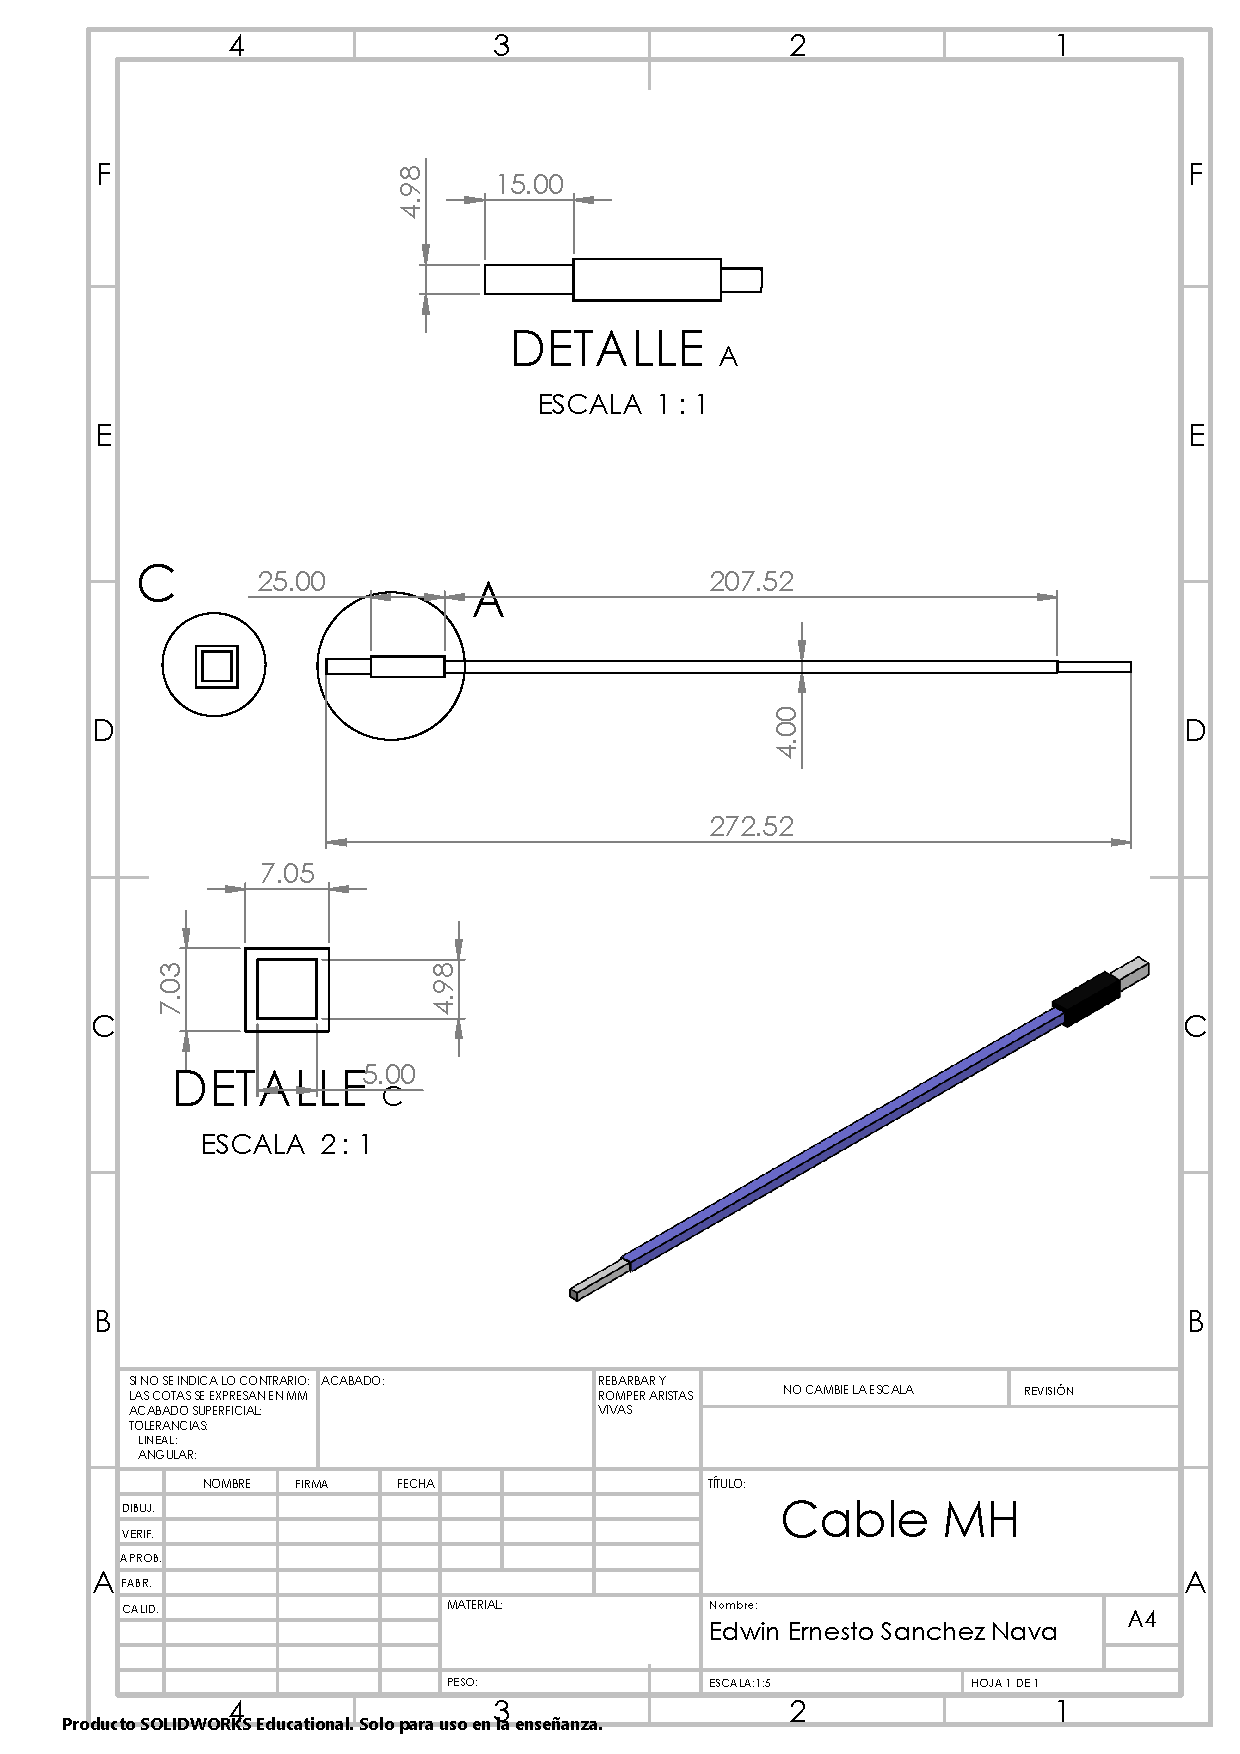
\includegraphics[width=.135\textwidth]{30/img/Cable MH.PNG} & \includegraphics[width=.135\textwidth]{30/img/Cable MH hoja.PNG} \\
        \hline
        Resistencia & 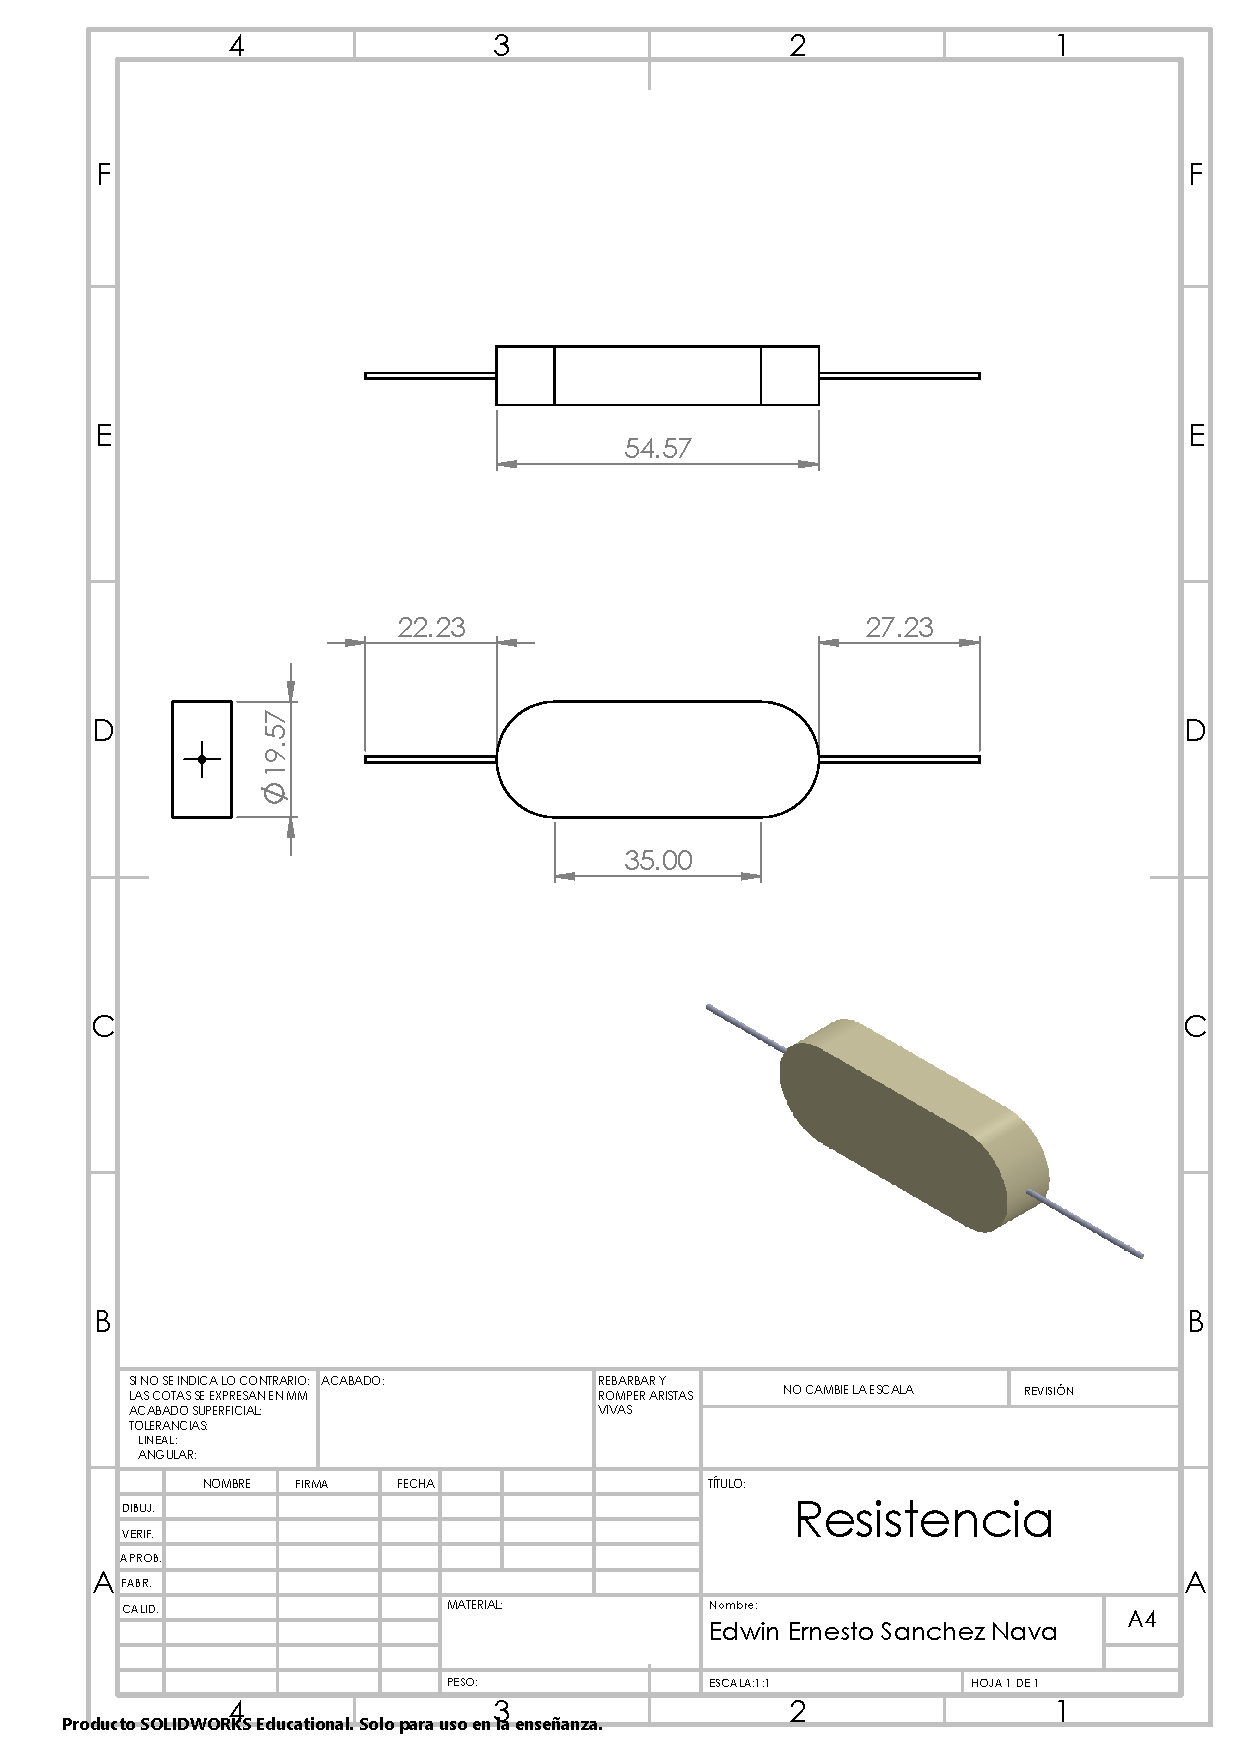
\includegraphics[width=.135\textwidth]{30/img/resistencia.PNG} & \includegraphics[width=.135\textwidth]{30/img/resistencia hoja.PNG} \\
        \hline
        Cable MM & 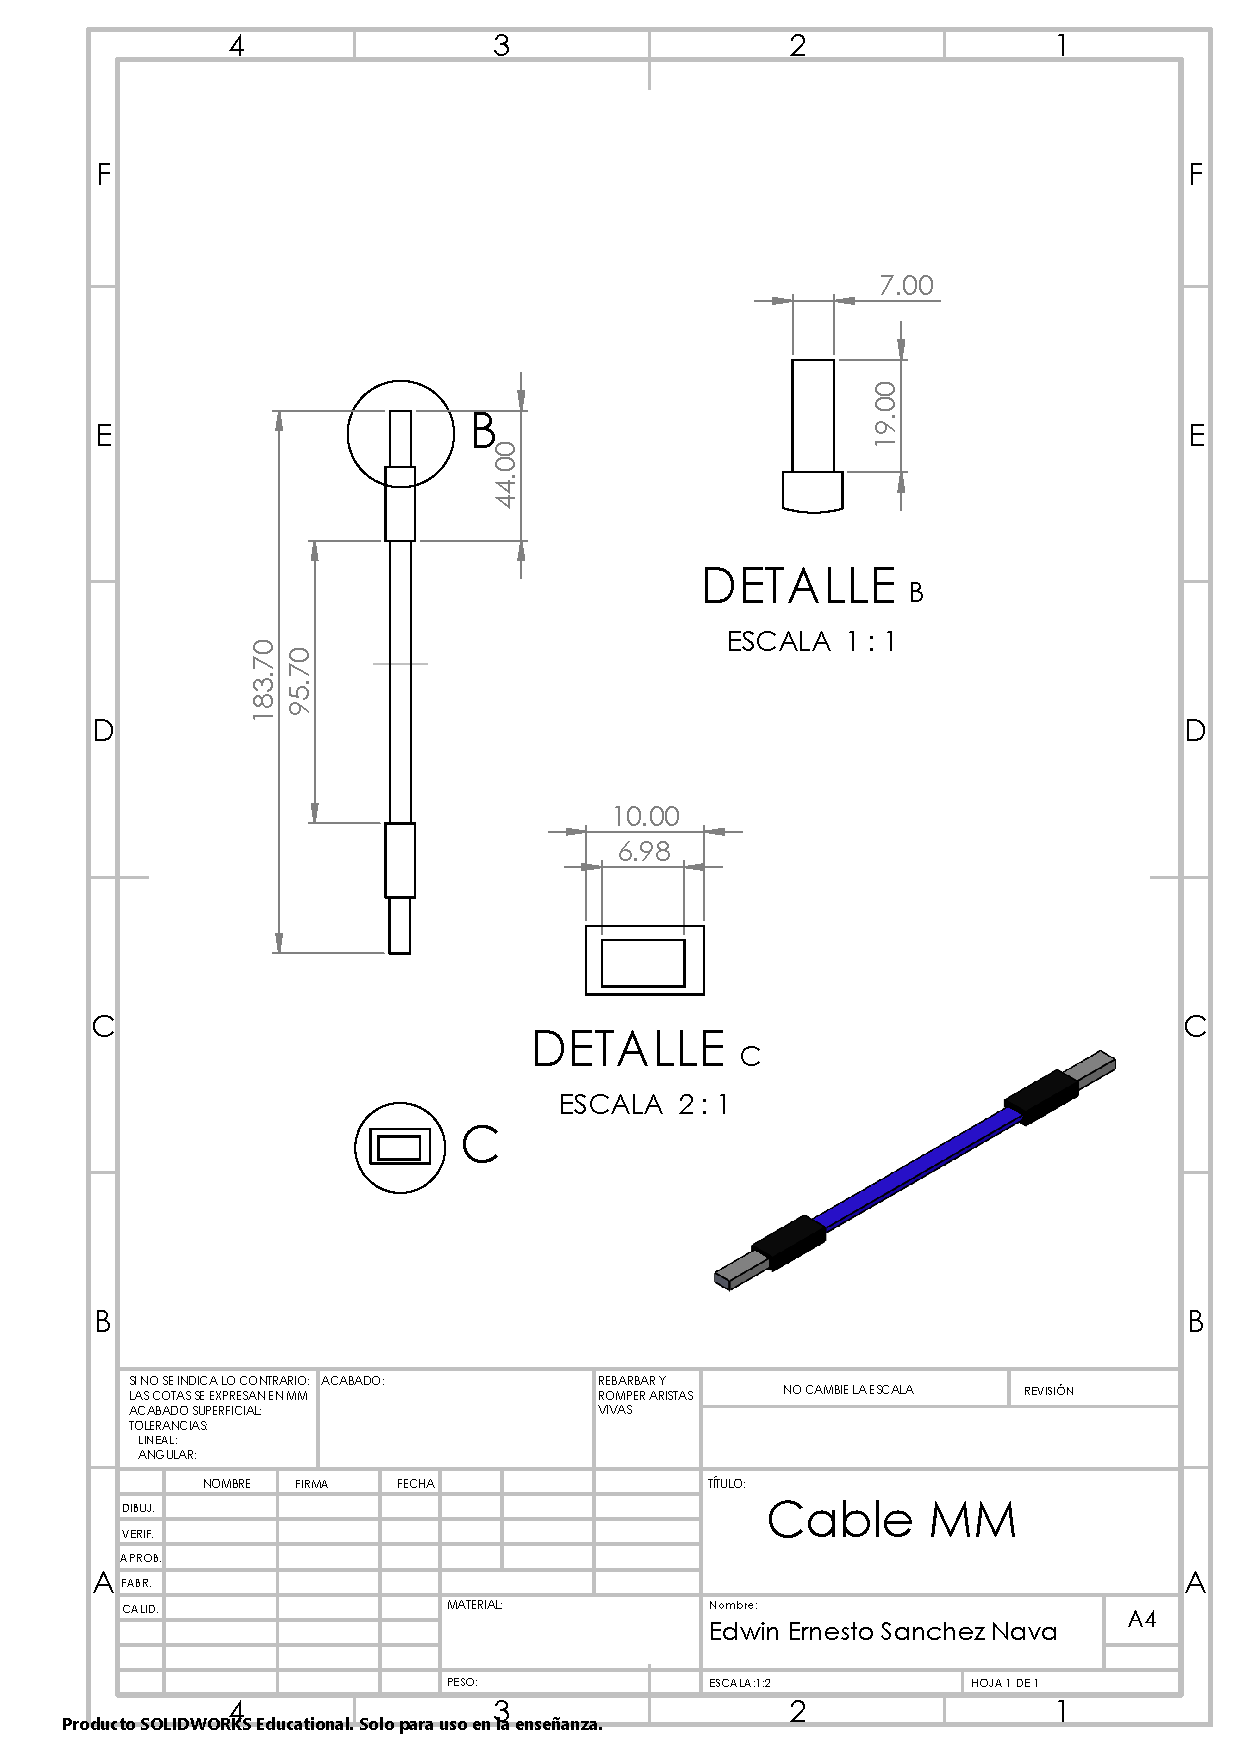
\includegraphics[width=.0650\textwidth]{30/img/Cable MM.PNG} & \includegraphics[width=.135\textwidth]{30/img/Cable MM hoja.PNG} \\
        \hline
        LCD & 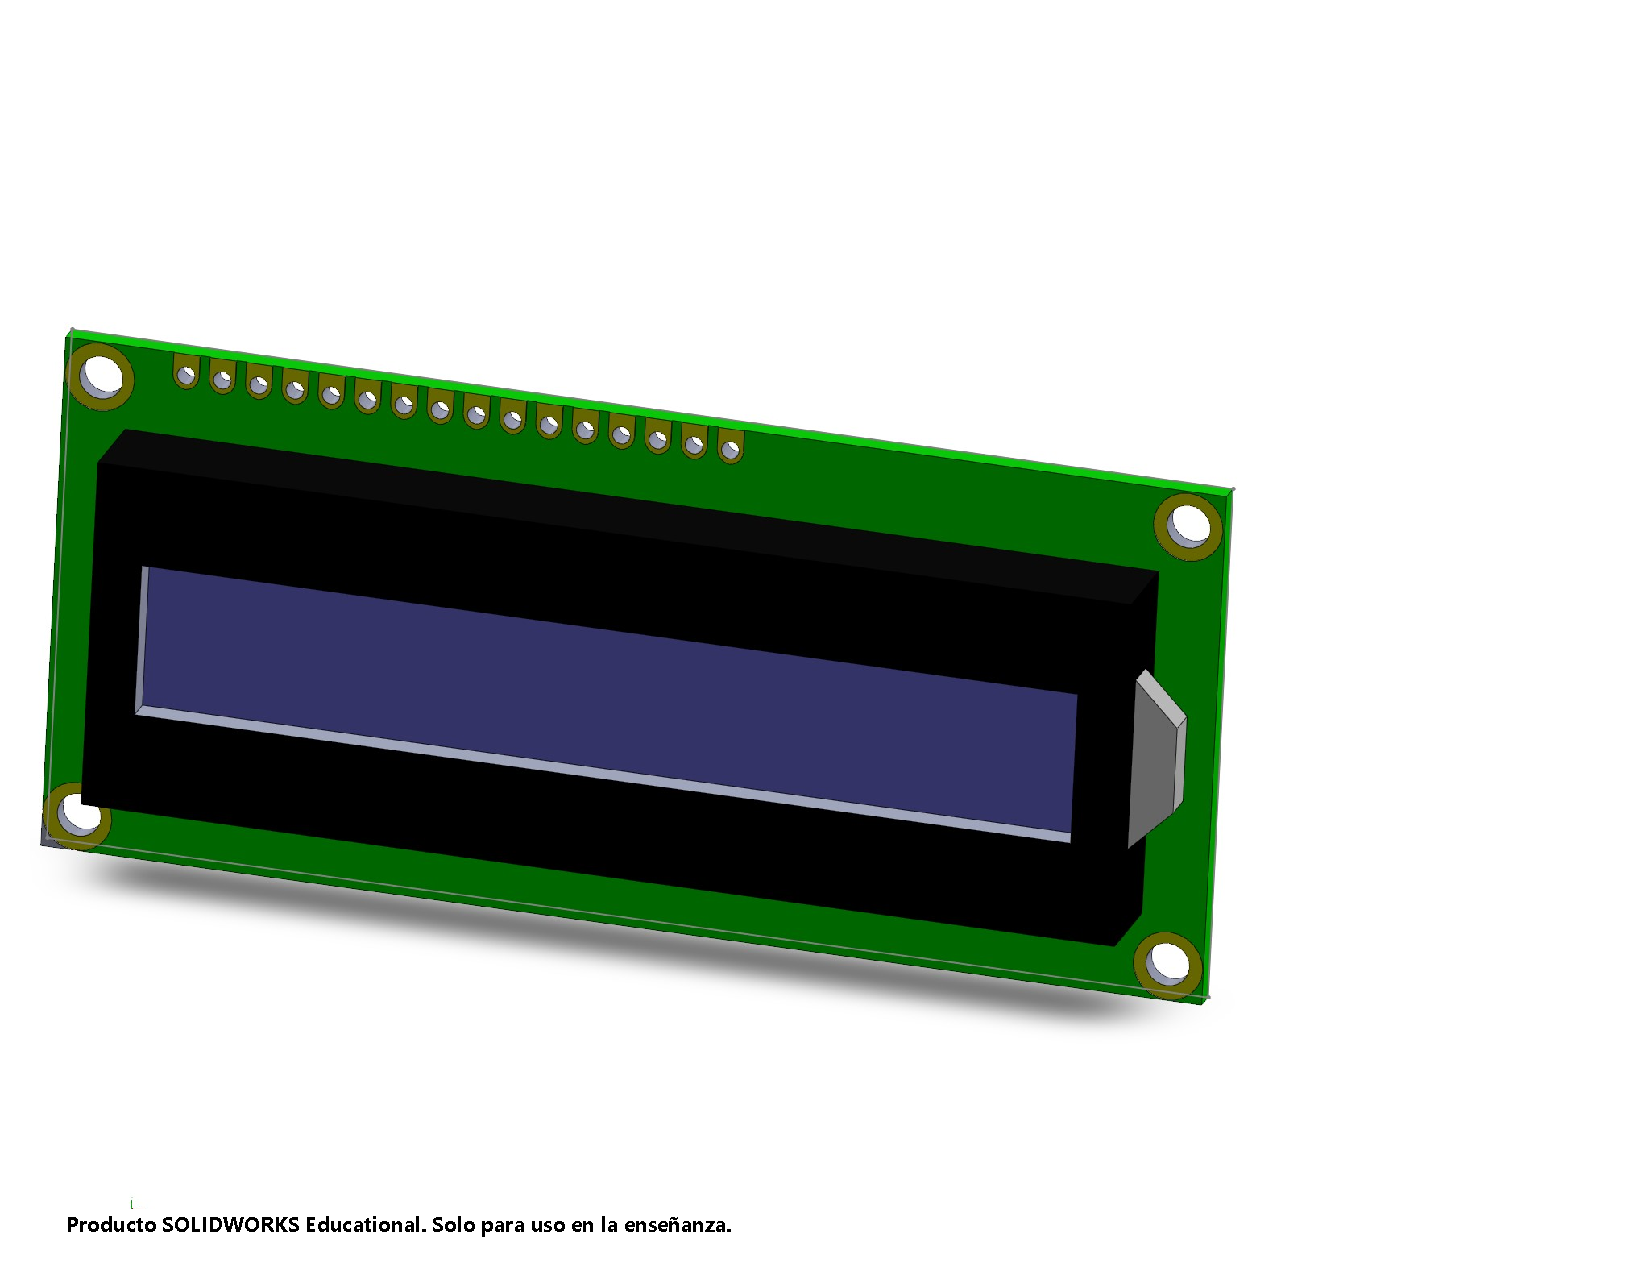
\includegraphics[width=.135\textwidth]{30/img/Lcd.PNG} & \includegraphics[width=.135\textwidth]{30/img/LCD hoja.PNG} \\
        \hline
        Potenciómetro & 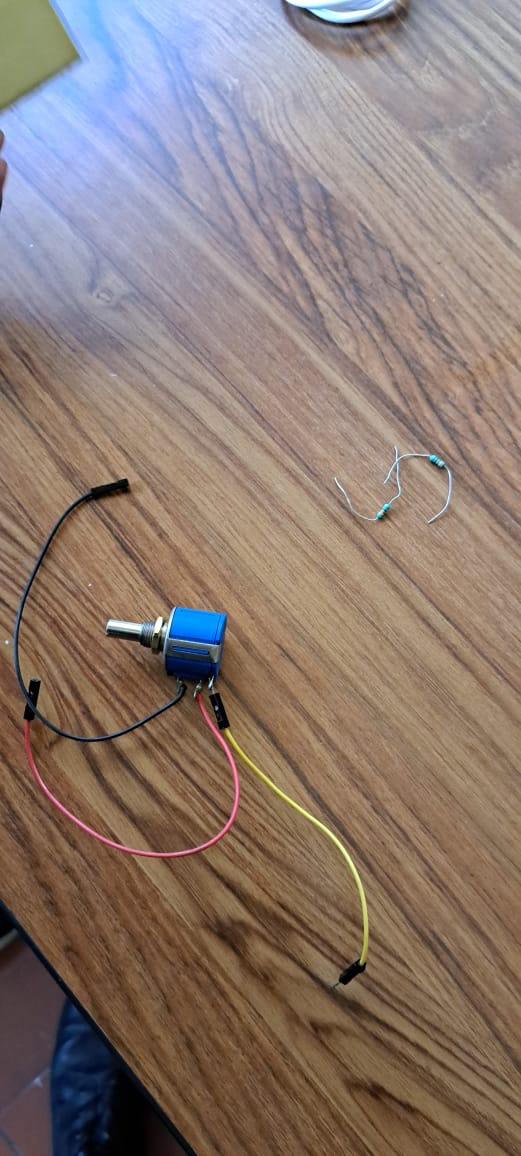
\includegraphics[width=.135\textwidth]{30/img/potenciometro.PNG} & \includegraphics[width=.135\textwidth]{30/img/Potenciometro hoja.PNG} \\
        \hline
        \end{tabular}
        \caption{Material}
        \label{tab:my_label}
    \end{table}
        % Ejemplo
        %  @Article{article,
        % 	author = "Author1 LastName1 and Author2 LastName2 and Author3 LastName3",
        % 	title = "Article Title",
        % 	volume = "30",
        % 	number = "30",
        % 	pages = "10127-10134",
        % 	year = "2013",
        % 	doi = "10.3389/fnins.2013.12345",
        % 	URL = "http://www.frontiersin.org/Journal/10.3389/fnins.2013.12345/abstract",
        % 	journal = "Frontiers in Neuroscience"
        % }
    
        % @book{book,
        %   author    = {Author Name}, 
        %   title     = {The title of the work},
        %   publisher = {The name of the publisher},
        %   address   = {The city},
        %   year      = 1993,
        % }
    
        % @incollection{chapter,
        %   author       = {Bauthor Surname}, 
        %   title        = {The title of the work},
        %   editor       = {Editor Name},
        %   booktitle    = {The title of the book},
        %   publisher    = {The name of the publisher},
        %   address      = {The city},
        %   year         = 2002,
        %   pages        = {201-213},
        % }
    
        % @InProceedings{conference,
        %   author = {Cauthor Name and Dauthor Surname and Fauthor LastName},
        %   title = {The title of the work},
        %   booktitle = {The title of the conference proceedings},
        %   year = 1996,
        %   publisher = {The name of the publisher},
        %   editor = {Editor Name1 and Editor Name2},
        %   pages = {41-50},
        % }
    
        % @book{cho,
        %   author       = {Gauthor Name1}, 
        %   title        = {The title of the work},
        %   publisher = {Country code and patent number},
        %   address      = {Patent Country},
        %   year = 2013
        % }
    
        % @book{patent,
        %   author    = {Hauthor Surname1}, 
        %   title     = {The title of the work},
        %   publisher = {Patent number},
        %   address   = {Patent country},
        %   year      = 2010,
        % }
    
        % % please use misc for datasets
        % @misc{dataset, 
        % 	author = "Author1 LastName1 and Author2 LastName2 and Author3 LastName3",
        % 	title = "Data Title",
        % 	year = "2011",
        % 	doi = "10.000/55555",
        % 	URL = "http://www.frontiersin.org/",
        % }
    
        \bibliographystyle{ieeetr}
        \bibliography{30/referencias}